\section{Challenges for imaging MeerKAT data} \label{meerkat}
New interferometers like MeerKAT put additional challenges on the image reconstruction problem. First, the new instrument produce a new magnitude of data, forcing reconstruction algorithms to be highly scalable and distributable. Second, the more sensitive instruments with large field of view amplify effects which were negligible in older instruments, like non-coplanar baselines or the ionosphere.

Compressed sensing has to be able to work with these issues somehow. Solutions all in the context of the major cycle, a new architecture may need to handle effects differently. Hopefully in a manner that is at least as efficient.

In this work, the effects of non-coplanar baselines gets handled in more detail. The effect has a neat mathematical notation, it adds a third fourier component to the measurement equation, but breaks the two dimensional fourier relationship introduced in section \ref{intro:basic}. 

Calibration used to be a task before image reconstruction.
Calibration gets not explicitly handled here, but it is important to keep in mind. For older interferometers, the data was calibrated before image reconstruction. With the advent of self-calibration, the image reconstruction is also used to improve calibration. MeerKAT requires more calibration parameters, so an image reconstruction algorithm has to be able to calibrate, or it is not interesting.



Further issues that do not get handled here
\begin{itemize}
	\item (Beam Pattern, A Projection)
	\item Full polarization
	\item Wide band imaging
\end{itemize}

There are several challenger for imaging meerkat data. One problem is the new amount of data.

terabytes of measurements. Large image size 32k squared are the obvious problems to solve. Distributing the problem is not part of this work.

 In this work, it is focused on Wide field of view issue. 







\subsection{Wide Field of View Imaging and the third Fourier Component} \label{meerkat:wof}
In wide field of view imaging, the simplifications we could make from the basic measurement equation \eqref{intro:basic} do not hold. The Visibility space of an interferometer actually has a third $w$-component. This leads us to the wide field of view measurement equation \eqref{meerkat:ftsphere}

\begin{equation}\label{meerkat:ftsphere}
V(u, v, w) = \int\int \frac{I(x, y)}{\sqrt{1 - x^2 - y ^2}} e^{2 \pi i [ux+vy+ w(\sqrt{1 - x^2 - y ^2} - 1)]} \: dx \: dy
\end{equation}

For a small field of view, the term  $\sqrt{1 - x^2 - y ^2} \approx 1$, which simplifies to our original \eqref{intro:basic}, we can ignore the $w$-term and use the two dimensional Fourier transform. For wide field of view however, the $w$-component cannot be ignored. The figure \ref{meerkat:wcorrection} shows the effect of ignoring $w$. The image gets continually more distorted away from the center. Emissions at the edges of the image get "torn" apart.


\begin{figure}[h]
	\centering
	\begin{subfigure}[b]{0.45\linewidth}
		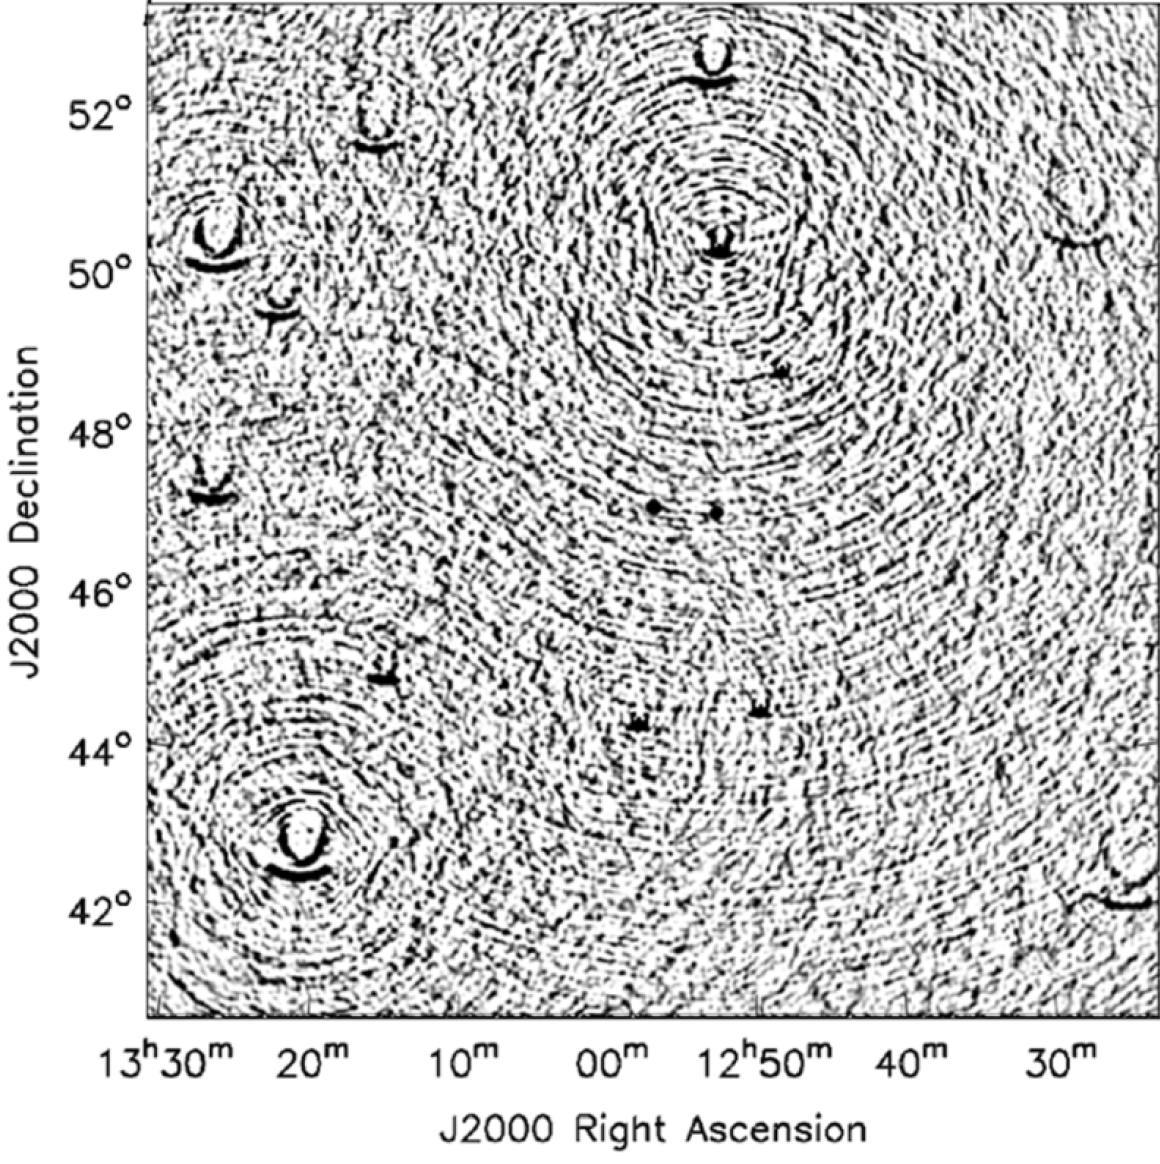
\includegraphics[width=\linewidth]{./chapters/03.challenges/w-no-correction.png}
		\caption{2D Fourier Transform.}
		\label{meerkat:2dfft}
	\end{subfigure}
	\begin{subfigure}[b]{0.45\linewidth}
		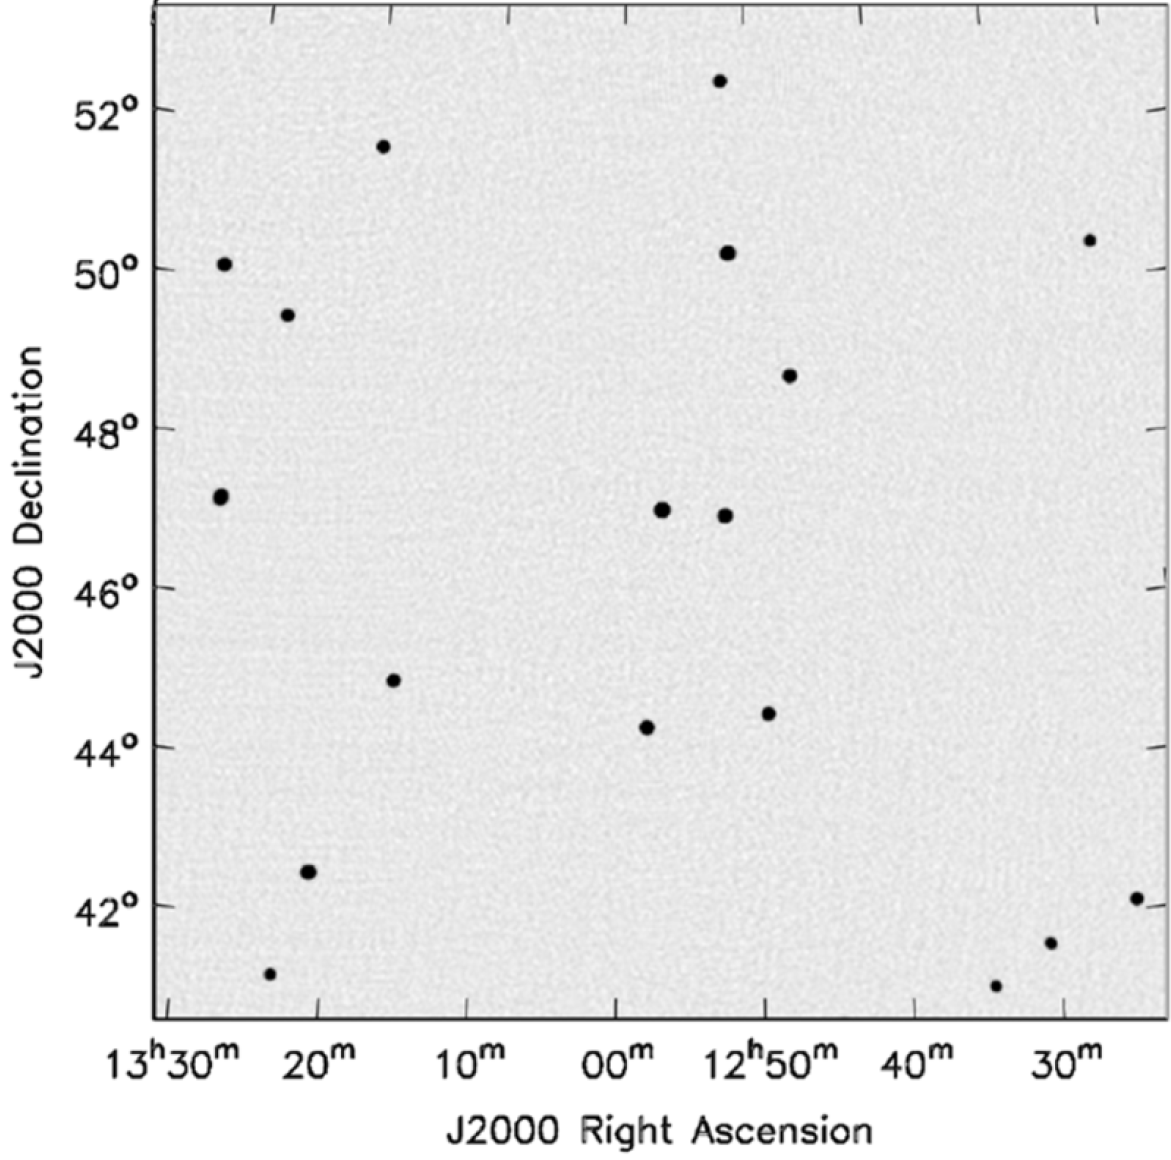
\includegraphics[width=\linewidth]{./chapters/03.challenges/w-correction.png}
		\caption{Fourier Transform with $w$-correction.}
		\label{meerkat:wcorrection}
	\end{subfigure}
	\caption{Celestial sphere distortion on simulated data. Source: \cite{cornwell2008noncoplanar}}
	\label{meerkat:wdistortion}
\end{figure}

We find the reason for why it distorts the edges, if we look at the measurement equation \eqref{meerkat:ftsphere} in detail. We see that the image $I(x,y)$ still two dimensional, even with a three dimensions in Visibility space. The observed image of the interferometer is not on a flat plane, but on a curved surface(hence the $w$-component)\cite{mcewen2011compressed}. More precisely, the instrument looks at the inside wall of the celestial sphere. The two dimensional Fourier transform approximates the sphere with a flat plane, where the tangent point is typically the image center. The further away we move from the tangent point, the more distortion gets added by the curvature, represented by the term $\sqrt{1 - x^2 - y ^2}$. The curve adds a phase shift the further away we move from the tangent point. If the reconstruction algorithm ignores the $w$-component for a wide field of view, the phase-shift gets severe enough to decorrelate the Visibilities, "tearing" apart the image structures of \eqref{meerkat}.

In the context of MeerKAT, the reconstruction algorithm has to handle the $w$-term in an efficient manner. The third Fourier breaks the two dimensional relationship between image and Visibilities, which keeps us from using the non-uniform FFT. In the Major Cycle architecture, $w$-stacking is the state-of-the-art way of correcting for the $w$-component efficiently. Since this project explores different architecture, we may need to find another way of correcting for the $w$-term.


\subsubsection{State of the art: $w$-stacking algorithm and WSCLEAN}
$w$-stacking\cite{pratley2018fast} is the current state-of-the-art approach for $w$-corrections. It is implemented in the WSCLEAN software package and is the current go-to algorithm for MeerKAT reconstructions. With $w$-stacking, we can again use the two dimensional non-uniform FFT for efficient transformations between image and Visibilities.

\begin{wrapfigure}{r}{0.7\textwidth}
	\centering
	\vspace{-10pt}
	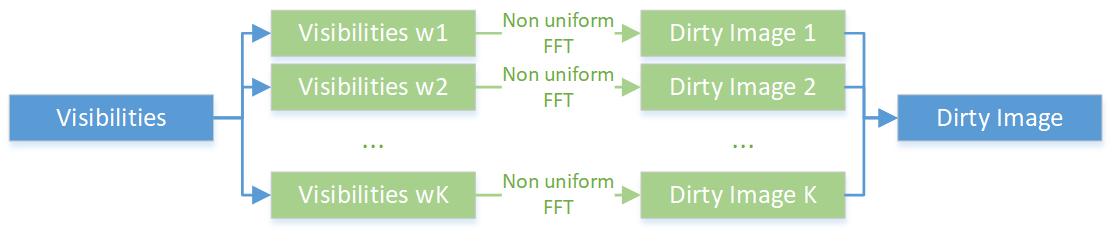
\includegraphics[width=1.0\linewidth]{./chapters/03.challenges/w-stacks.png}
	\caption{The Major Cycle Framework}
	\label{meerkat:w-stacks}
	\vspace{-10pt}
\end{wrapfigure}

$w$-stacking, shown in figure \ref{meerkat:w-stacks} replaces the non-uniform FFT operation from figure \ref{intro:major}. It groups the Visibilities with similar $w$-term into the same layer. Multiple layers are then stacked and transformed independently with the non-uniform FFT. For each stack, the $w$-correction is performed for the center $w$-component. The last step is summing over all stacked images, giving us the final dirty image. At this point a deconvolution algorithm like CLEAN can deconvolve the dirty image. 

After the deconvolution, the whole process is reversed. The image gets copied back into the stacks, the $w$-correction gets reversed and the non-uniform FFT calculates the Visibilities per stack.

If we choose uses as many stacks as Visibilities, we end up with an exact $w$-corrections. In pracice, many Visibilities have a similar $w$-term. $w$-stacking approximates the correction and allows the Major Cycle to distribute the forward- and backwards Fourier transform to a certain extend.

\subsection{Self-Calibration}
Complex gain term. Corrects amplitude and phase. 

Traditional Calibration

A calibration source close by, with a known brightness. Phase and amplitude calibration was done before image reconstruction. For older interferometers, there was a very limited number of calibration terms to solve.


but again effects of wide field of view also increase the number of necessary calibration terms. The advent of self calibration, in which the image reconstruction was used to solve for both, the observed image and the calibration of the instrument.

Self calibration with the major cycle algorithm and a CLEAN deconvolution.

Initial phase calibration
Shallow clean
phase calibration
deep clean
phase and amplitude calibration
deep clean
reconstruction






